\documentclass{llncs}
%\pagestyle{plain}

\usepackage[cmex10]{amsmath}
\usepackage{amssymb}
\usepackage{array}
\usepackage{bm}
\usepackage{graphicx}
\usepackage{epstopdf}
\usepackage[hang]{subfigure}
\usepackage{import}
\usepackage{booktabs}
\usepackage{tabularx}
\usepackage{pdfpages}
\usepackage{epstopdf}
\graphicspath{{figures/}}
\usepackage{wrapfig}
\usepackage[export]{adjustbox}
\usepackage[font=scriptsize]{caption}
\usepackage{mwe}


%\usepackage[colorlinks=true,linkcolor=blue,citecolor=blue,urlcolor=black]{hyperref}
\usepackage{algorithm, algpseudocode}
%\algsetup{linenosize=\scriptsize}

% Commenting functionality
%\usepackage{todonotes}
%\reversemarginpar

\newcommand{\brs}[1]{\left[{#1}\right]} %square bracets
\newcommand{\brr}[1]{{\left({#1}\right)}} %round bracets
\newcommand{\brf}[1]{\left\lbrace{#1}\right\rbrace} %figure bracets
\newcommand{\brabs}[1]{\left\vert{#1}\right\vert} %absolute bracets
\newcommand{\norm}[2]{\left\|{#1}\right\|_{#2}} %norm_*

\newcommand{\I}[1]{I\!\left[{#1}\right]} %Robustness criterion I[*]
\newcommand{\Iq}[1]{I_q\!\left[{#1}\right]} %Robustness criterion I_q[*]
\newcommand{\Ic}[1]{I_c\!\left[{#1}\right]} %Robustness criterion I_c[*]

\newcommand{\vx}{\mathbf{x}} % vector x
\newcommand{\vy}{\mathbf{y}} % vector y
\newcommand{\vX}{\mathbf{X}} % vector X
\newcommand{\vf}{\mathbf{f}} % vector f
\newcommand{\vz}{\mathbf{z}} % vector z
\newcommand{\vZ}{\mathbf{Z}} % vector Z
\newcommand{\vw}{\mathbf{w}} % vector w
\newcommand{\vd}{\mathbf{d}} % vector d
\newcommand{\vp}{\mathbf{p}} % vector p
\newcommand{\vP}{\mathbf{P}} % vector P
\newcommand{\vu}{\mathbf{u}} % vector u
\newcommand{\vU}{\mathbf{U}} % vector U
\newcommand{\DSet}{\mathcal{D}} % Set D
\newcommand{\NSet}{\mathcal{N}} % Set N
\newcommand{\XSet}{\mathcal{X}} % set X
\newcommand{\ZSet}{\mathcal{Z}} % set Z
\newcommand{\SSet}{\mathcal{S}} % set S
\newcommand{\ISet}{\mathcal{I}} % set I
\newcommand{\Pref}{\mathcal{P}} % Preferences set P

\DeclareMathOperator*{\argmin}{\arg\!\min}
\DeclareMathOperator*{\argmax}{\arg\!\max}


\begin{document}
\title{sParEGO -- A Hybrid Optimization Algorithm for Expensive Uncertain Multi-Objective Optimization Problems}
\author{Jo\~{a}o A. Duro\inst{1} \and Robin C. Purshouse\inst{1} \and Shaul Salomon\inst{1,2} \and Daniel C. Oara\inst{1} \and Visakan Kadirkamanathan\inst{1} \and Peter J. Fleming\inst{1}}
\institute{University of Sheffield, UK \email{\{j.a.duro,r.purshouse\}@sheffield.ac.uk}
\and ORT Braude College of Engineering, Israel, \email{shaulsal@braude.ac.il}}

\maketitle

\begin{abstract}
Evaluations of candidate solutions to real-world problems are often expensive to compute, are characterised by uncertainties arising from multiple sources, and involve simultaneous consideration of multiple conflicting objectives. Here, the task of an optimizer is to find a set of solutions that offer alternative robust trade-offs between objectives, where robustness comprises some user-defined measure of the ability of a solution to retain high performance in the presence of uncertainties. Typically, understanding the robustness of a solution requires multiple evaluations of performance under different uncertain conditions -- but such an approach is infeasible for expensive problems with a limited evaluation budget. To overcome this issue, a new hybrid optimization algorithm for expensive uncertain multi-objective optimization problems is proposed. The algorithm -- sParEGO -- uses a novel uncertainty quantification approach to assess the robustness of a candidate design without having to rely on expensive sampling techniques. Hypotheses on the relative performance of the algorithm compared to an existing method for deterministic problems are tested using two benchmark problems, and provide preliminary indication that sParEGO is an effective technique for identifying robust trade-off surfaces.
\keywords{Expensive optimization, surrogate-based optimization, robust optimization, multi-objective optimization}
\end{abstract}

\section{Introduction}

The ability of simulations to predict the performance of a candidate design is constantly increasing. While some simulations can produce high-fidelity outputs relatively quickly, a typical mesh-based simulation can run for several hours, and even days. Even if a design team has access to supercomputing resources, the extensive run-time still implies that perhaps only a few hundred candidate designs can be explored using high-fidelity modelling resources. Unfortunately, conventional multi-objective optimization algorithms implemented in commercial packages typically require tens of thousands of function evaluations to converge on a high quality solution~\cite{Zhou2011Multiobjective}. Therefore, the search for a promising design using expensive evaluation functions on a limited computational budget poses a great challenge.

To exacerbate this problem, optimizing for a robust solution is itself a computationally demanding task. In order to gain confidence over the robustness of a solution to uncertainties, the statistical properties of the expected solution's performance must be quantified. In a world where the complexity of the high-fidelity models essentially produces a black-box mapping of inputs to outputs, such statistical properties would typically be found through repeated evaluation of the same solution using those high-fidelity models. However, repeatedly sampling a single candidate design is computationally expensive.

To address the above, we propose a framework for expensive uncertain multi-objective optimization problems (MOPs). The key aims are to: (i) exploit expensive, black-box evaluation function for a candidate design; (ii) account for multiple sources of uncertainty, such as fidelity of evaluation functions and manufacturing tolerances; and (iii) provide an understanding of the risk and opportunity trade-offs between candidate designs with respect to a given robustness metric. To achieve this the framework leverages ParEGO~\cite{Knowles2006ParEGO}, an algorithm for multi-objective optimization, which has been demonstrated to provide good results for optimization runs limited to a small number of function evaluations. ParEGO itself is a multi-objective extension to Jones et al.'s~\cite{Jones1998Efficient} seminal efficient global optimization (EGO) algorithm for single-objective problems. The main limitation of ParEGO is that it has not been designed to handle problems featuring uncertainty (although
there is some evidence that it can perform favourably in noisy environments~\cite{knowles2009noisy}). Therefore a fundamental part of the framework is how ParEGO can be extended to consider evaluation functions as samples of random variates. We refer to this new algorithm as \emph{stochastic ParEGO} or \emph{sParEGO}. 

In the remainder of this paper, first the robustness metric used is described in Section~\ref{sec:robustness_metric}, and the proposed framework is presented in Section~\ref{sec:framework}. The hypotheses on the relative performance of the algorithm are introduced in Section~\ref{sec:test_suite}. The experimental settings and findings are in Section~\ref{sec:results}. The paper concludes with Section~\ref{sec:conclusion}.

\section{Threshold-based robustness metric}\label{sec:robustness_metric}

A general single-objective robust optimisation problem can be formulated as:
\begin{align}
\min_{\vx\in\Omega} S=\vf\brr{\vx,\vU}.
\label{eq:rev:robust}
\end{align}
Here, $\vx=[x_1,\ldots,x_{n_x}]$ is a vector of $n_x$ decision variables in a feasible domain $\Omega$, $\vU$ is a vector of random variables that includes all the uncertainties associated with the optimisation problem. These uncertainties may be an outcome of manufacturing tolerances, a noisy environment, evaluation inaccuracies etc. A single scenario of the variate $\vU$ is denoted as $\vu$. Since uncertainties are involved, the scalar objective $S$ is also a random variate, where every scenario of the uncertainties, $\vu$, is associated with an objective value $s$.

In a robust optimisation scheme, the random objective value is replaced with a robustness criterion, denoted by the indicator $\I{S}$. Several criteria are commonly used in the literature, which can be broadly categorised into three main approaches:
\begin{enumerate}
\item \textbf{Worst-Case Scenario.} The worst objective vector, considering a bounded domain in the neighbourhood of the nominal values of the uncertain variables.
\item \textbf{Aggregated Value.} An integral measure of robustness that amalgamates the possible values of the uncertain variables (e.g. mean value or variance).
\item \textbf{Threshold Probability.} The probability for the objective function to be better than a defined threshold.
\end{enumerate}

In our framework the third approach, suggested by Beyer and Sendhof~\cite{Beyer2007}, is used. A threshold $q$ is considered as a satisficing performance for the objective value $s$. When $s$ is uncertain, denoted by the random variable $S$, the probability for $S$ to satisfy the threshold level can be seen as a confidence level $c$. For a minimization problem this can be written as:
\begin{align}
c\brr{S,q}=\text{Pr}\brr{S<q}.
\label{eq:confidence}
\end{align}
A robustness indicator used in this paper is based on minimization of the threshold $q$ for a pre-defined confidence level $c$, meaning that the confidence in the resulting performance can be specified (e.g.~by a decision-maker).

A stochastic unconstrained multi-objective optimization problem (MOP), which is the focus of this study, can be formulated as:
\begin{align}
\label{eq:mop}
        \min_{\vx\in\Omega} \vZ=\vf\brr{\vx, \vU}.
\end{align}
where $\vZ$ is a multivariate random vector of $n_z$ performance criteria, and $\vf$ is a set of functions mapping from decision-space to objective-space. Due to uncertainties over the problem parameters or the mapping functions themselves, every evaluation of the same decision vector may result in a different realisation of the objective vector $\vz=[z_1,\ldots,z_{n_z}]$.

\section{The Framework of the sParEGO Algorithm}\label{sec:framework}

%\subsection{General Framework}

sParEGO is a surrogate-based multi-objective optimization algorithm for dealing with stochastic MOPs. The algorithm shares many similarities with ParEGO including the ability to approximate expensive MOPs over a realistically small number of function evaluations. The main idea is that the uncertain distribution in objective space of every candidate solution is not quantified through uncertainty quantification methods (e.g. Monte Carlo sampling). Instead, every solution is evaluated once, and the distribution is approximated based on the performance of nearby solutions. A pseudo-code of sParEGO is presented in Algorithm~\ref{alg:sParEGO} and a general description of its working principles is as follows.

The decision variables and objectives are normalised to non-dimensional units in the following manner:
\begin{align}
 \tilde{x}_i &= (x_i-x_i^l)/(x_i^u - x_i^l),~i=1,\ldots,n_x,\\
 \tilde{z}_j &= (z_j-z_j^*)/(z_j^n - z_j^*),~j=1,\ldots,n_z,
\end{align}
where $x_i^u$ and $x_i^l$ are the upper and lower boundaries of the $i^{th}$ decision variable, $z_j^n$ and $z_j^*$ are the $j^{th}$ components of the estimated nadir and ideal vectors, and the tilde accent represents a normalised, dimensionaless variable. The normalised values are used for all operations within the algorithm. Before a candidate design is evaluated, it is re-scaled to the natural dimensions.

sParEGO decomposes the overall MOP into a number of single-objective problems by using a set of (reference) direction vectors to guide the search towards different regions of the Pareto front\footnote{More details about the decomposition strategy are provided in Section~\ref{sec:decomposition}.}. The set of all direction vectors is denoted by $\DSet$ (Line 1). The direction vectors are picked (one at the time) based on their sequence in the set $\DSet$. Once all direction vectors have been traversed by the optimizer the vectors in the set $\DSet$ are shuffled (Line 5). This prevents any bias that might arise due to repeatedly using the same sequence of direction vectors during the entire optimization process. 

The procedure used to generate the initial set of solutions ($\XSet$) is described in Section~\ref{subsec:initialisation} (Line 2). Following this, all solutions in the set $\XSet$ are evaluated and their performance is stored in the set $\ZSet$ (Line 3). The ideal and nadir vectors are then updated (Line 7). A scalar fitness value is obtained for each solution by using a scalarising function as mentioned in Section~\ref{sec:decomposition} (Line 8). The robustness indicator values of the solutions are estimated and stored in the set $\ISet$ (Line 9), and these are used to construct a surrogate model (Line 10). A search procedure is then conducted over the model to find a solution $\vx^\text{new}$ that optimizes the given robustness indicator based on the concept of expected improvement (Line 11). A new solution $\vx^\text{pert}$ is generated by applying a perturbation to $\vx^\text{new}$ (Line 12). This ensures that all generated solutions have at least one nearby solution. The new solutions are added to $\XSet$ (Line 13) and, once evaluated, their performance is stored in $\ZSet$ (Line 14). The algorithm goes back to Line 4 and the procedure repeats itself until a stopping criteria is satisfied.

The robustness indicator values of the solutions are estimated based on the procedure in Line 17. The first step is to identify, for each solution, all the nearby solutions. For this, we define the concept of neighbourhood and consider that two solutions are neighbours if their distance in normalised decision-space is within a user-defined neighbourhood distance $\delta$ (Line 19). The statistical properties of the performance of a solution is approximated from the other neighbouring solutions (Line 23). Finally, the robustness indicator values of the solutions are estimated for a given robustness criterion $I$ (Line 24).

\begin{algorithm}
\scriptsize
\caption{\textsc{sParEGO} Pseudo-code}
\label{alg:sParEGO}
\begin{algorithmic}[1]
        \Statex \textbf{Parameters:} initial set size $n_\text{init}$, surrogate model maximum set size $n_\text{max}$, maximum distance between newly generated solutions $\delta_\text{pert}$, robustness criterion $I$, neighbourhood distance $\delta$
        \State $\DSet \leftarrow$ set of all reference direction vectors \Comment{Equation~\ref{eq:simplex_lattice_design} (Section~\ref{sec:decomposition})}
        \State $\XSet \leftarrow$ generate initial set of solutions using $n_\text{init}$ and $\delta_\text{pert}$ \Comment{Section~\ref{subsec:initialisation}}
        \State $\ZSet \leftarrow \vf\brr{\XSet}$ \Comment{evaluate the initial set}
        \While{stopping criteria not satisfied}
                \State Shuffle the set $\DSet$
                \ForAll{$\vd\in\DSet$}
                        \State update ideal and nadir vectors
                        \State $\SSet \leftarrow$ calculate scalar fitness value of all solutions \Comment{Equation~\ref{eq:scalarising_function} (Section~\ref{sec:decomposition})}
                        \State $\ISet \leftarrow$ \Call{RobustnessApproximation}{$\XSet,\SSet,\delta$} \Comment{Sections~\ref{subsec:uncertainty_quantification} and~\ref{subsec:robustness_indicators}}
                        \State $model \leftarrow$ fit a Surrogate model to the indicator values $\ISet$ using $n_\text{max}$ \Comment{Section~\ref{subsec:Kriging}}
                        \State $\vx^\text{new} \leftarrow$ maximize the expected improvement based on $model$
                        \State $\vx^\text{pert} \leftarrow$ add a neighbour to $\vx^\text{new}$ using $\delta_\text{pert}$ \Comment{Section~\ref{subsec:Kriging}} 
                        \State $\XSet \leftarrow \XSet \cup \brf{\vx^\text{new}, \vx^\text{pert}}$
                        \State $\ZSet \leftarrow \ZSet \cup \brf{\vf\brr{\vx^\text{new}}, \vf\brr{\vx^\text{pert}}}$ \Comment{evaluate the new solutions}
                \EndFor
        \EndWhile
%\Statex
\Procedure{RobustnessApproximation}{$\XSet,\SSet, \delta$}
 \ForAll{$\vx_i\in\XSet$}
  \State update the neighbourhood $\NSet(\vx_i)$ for a given $\delta$ \Comment{Equation~\ref{eq:neighbourhood} (Section~\ref{subsec:uncertainty_quantification})}
 \EndFor
 \State $\ISet \leftarrow \emptyset$
 \ForAll{$\vx_i\in\XSet$}
  \State approximate the distribution of $S_i$ \Comment{Section~\ref{subsec:uncertainty_quantification}}
  \State calculate robustness indicator $\I{S_i}$ \Comment{Section~\ref{subsec:robustness_indicators}}
  \State $\ISet \leftarrow \ISet \cup \I{S_i}$
 \EndFor
 %\State \textbf{return} $\ISet$
\EndProcedure

\end{algorithmic}
\end{algorithm}

% \subsection{Parameters}\label{subsec:Parameters}
% \begin{itemize}
% \item $\delta$ -- Neighbourhood distance. Maximum distance between solutions to be considered as neighbours. Default value is $0.1 \sqrt{n_x}$.
% \item $n_\text{init}$ -- Size of initial population.
% \item $n_\text{indp}$ -- Portion of solutions in the initial population that are independently generated. Must be smaller or equal to $n_\text{init}/2$.
% \item $\delta_\text{pert}$ -- Maximum distance between newly generated solutions. Default value is $\delta / 2$.
% \item $c$ -- Desired level of confidence in the performance of the solutions.
% \item $n_\text{max}$ -- Maximum number of solutions to construct the Surrogate model.
% \end{itemize}

\subsection{Decomposition}\label{sec:decomposition}

A decomposition-based algorithm decomposes the MOP into a number of single-objective problems, each approaching the global trade-off surface from a different direction. The $i^\textrm{th}$ sub-problem is associated with a reference direction vector $\vd^i$ which is taken from the set $\DSet$. The set is constructed by using a Simplex Lattice design:
\begin{equation}
 \DSet = \left\{ \vd =[d_1,\ldots,d_{n_z}]~ |~ \sum_{j=1}^{n_z} d_j=1 \wedge   d_j\in \left\{\frac{0}{h},\frac{1}{h},\ldots,\frac{h}{h}\right\} \text{for all } j \right\},
 \label{eq:simplex_lattice_design}
\end{equation}
where $h$ is a parameter that defines the number of divisions for each objective.

Each sub-problem assigns a scalar fitness value to each solution. This is achieved by using a scalarising function $f(\vz,\vw)$ that maps an objective vector $\vz$ into a scalar value according to a vector of weights $\vw=[w_1,\ldots,w_{n_z}]$. The scalarising function used is the weighted Tchebycheff, which is given by:
\begin{equation}
 s = \max\limits_{1\leq i \leq n_z} \left\{ w_i z_i \right\}.
 \label{eq:scalarising_function}
\end{equation}
For a given direction vector $\vd$ there is a corresponding weighting vector that minimizes the scalarising function~\cite{bib:generational_distance}. The optimal weighting vector $\vw$ for the scalarising function in (\ref{eq:scalarising_function}) is defined as:
\begin{equation}
w_i=t_i \Big/ \sum_{i=1}^{n_z} t_i \text{ where } t_i = (d_i+\epsilon)^{-1}, ~i=1,\ldots,n_z, \text{ and } \sum_{i=1}^{n_z} w_i=1,
\end{equation}
where $\epsilon$ is a small number to prevent division by zero.

\subsection{Initialisation}\label{subsec:initialisation}

In sParEGO, the robustness assessment of a candidate design relies on the determination of its statistical properties, which in turn depends on the information of the neighbouring solutions. Hence, in order to support the robustness assessment from the beginning of the optimization process, for any solution in the inital set there is at least one nearby solution in desision-space. Let $n_{\text{init}}$ denote the size of the initial set, then the procedure is as follows:
\begin{enumerate}
 \item To provide a good coverage, a space-filling design technique (Latin Hypercube sampling) is used to generate a fraction of the total $n_{\text{init}}$. We suggest this fraction to be a quarter.
 
 \item For every existing solution in $\XSet$, another solution is generated by applying a random perturbation where the upper bound is within a hypersphere with a radius of $\delta_\text{pert}$.
 
 \item The rest of the solutions are generated by randomly selecting an existing solution from $\XSet$ and applying a perturbation as in the previous step. This step is repeated until the number of solutions in $\XSet$ is equal to $n_{\text{init}}$.
\end{enumerate}

The second step enforces that every solution has at least one neighbour. The third step seeds the initial population with neighbourhoods of different sizes.


\subsection{Uncertainty quantification}\label{subsec:uncertainty_quantification}

The most important difference between sParEGO and ParEGO is that the former assumes that the outcome of an evaluation function is a realization of a random variate. Therefore, the scalarised function value cannot be used directly to construct the surrogate model, and a utility indicator value is used instead. For every direction vector, the surrogate model is constructed to search for a design that will optimize a given robustness indicator (described in Section~\ref{subsec:robustness_indicators}). The guiding principle is to avoid having to repeatedly sample every candidate design to assess its statistical properties in objective-space. Instead, these properties (specifically, measures of central tendency and dispersion) are approximated from the available information of other candidate design evaluations.

\subsubsection{Approximation of the central tendency}

The stochasticity of the problem might originate from a variety of sources, including variations in decision-space. For this type of uncertainty, two designs with similar nominal values can be identical when realised. Therefore, the performance of a candidate design should be calculated from the performance of neighbouring designs as well. Two solutions $\vx_i$ and $\vx_j$ are considered as neighbours if their Euclidean distance in normalised decision-space is smaller than or equal to $\delta$, that is:
\begin{align}
\norm{\vx_i-\vx_j}{2}\leq\delta.
\end{align}
For a solution $\vx_i$ with a scalar fitness given by $s_i$, the statistical properties of the scalar fitness are approximated from the neighbouring solutions as follows:
First, the neighbourhood $\NSet(\vx_i)$ of the solution is defined\footnote{Note that according to~\eqref{eq:neighbourhood}, $\vx_i$ is included in the neighbourhood $\NSet(\vx_i)$.}:
\begin{align}
\NSet(\vx_i)=\brf{\vx_j\in \XSet \,\vert \,\norm{\vx_i-\vx_j}{2}\leq\delta}.
\label{eq:neighbourhood}
\end{align}
Next, the approximated mean function value, $\mu_s$, is derived from the neighbourhood.
Members that are closer to $\vx_i$ are given a larger weight, denoted as $v$ in Equation~\eqref{eq:neighbourhood_weights}, in approximating its properties.
Since the weight of most solutions in the neighbourhood is smaller than 1, the overall ``neighbourhood size'' $N_i$ is smaller than $\brabs{\NSet(\vx_i)}$:
\begin{align}
\label{eq:neighbourhood_weights}
v_j &= \frac{\delta-\norm{\vx_i-\vx_j}{2}}{\delta}, ~\forall \vx_j\in\NSet(\vx_i),\\
\label{eq:neighbourhood_size}
N_i &= \sum_{\vx_j\in\NSet(\vx_i)} v_j,\\
\label{eq:neighbourhood_mean}
\mu_{s,i} &= \frac{1}{N_i}  \sum_{\vx_j\in\NSet(\vx_i)} v_j s_j,
\end{align}
where $\mu_{s,i}$ is the approximated mean of the scalar fitness function for $\vx_i$.

\subsubsection{Approximation of the dispersion}

Once the expected mean is known, the expected value for the variance is calculated:
\begin{equation}
\sigma_{s,i}^2 = \frac{1}{N_i} \sum_{\vx_j\in\NSet(\vx_i)} v_j \brr{s_j - \mu_{s,i}}^2 .
\label{eq:neighbourhood_variance}
\end{equation}

An example is shown in Figure~\ref{subfig:indicator_estimation_1} for an optimization problem with a single decision variable where 5 solutions are divided into two neighbourhoods. The mean and variance of the scalar fitness function is estimated based on their scalar fitness values and their decision-space distance within the neighbourhood.

\begin{figure}
\centering
\subfigure[Estimation of the mean value and the variance from the neighbourhood]{
        \def\svgwidth{0.44\textwidth}
        \import{figures/}{indicator_estimation_1.pdf_tex}
        \label{subfig:indicator_estimation_1}
}
\hspace{1mm}
\subfigure[Assuming a normal distribution for $S$ according to $\mu_s$ and $\sigma_s$. The shaded area represents a confidence of $80\%$.]{
        \def\svgwidth{0.44\textwidth}
        \import{figures/}{indicator_estimation_2.pdf_tex}
        \label{subfig:indicator_estimation_2}
}
\caption{Approximation of the statistical properties, and estimation of robustness indicator $\Ic{\bullet}$.}
\label{fig:indicator_estimation}
\end{figure}

\subsection{Estimating the robustness indicator value}\label{subsec:robustness_indicators}

Once the mean and variance of the scalar fitness function have been estimated for every solution in the set, the random variable $S\brr{\vx}$ is assumed to follow a normal distribution. The robustness indicator is calculated for this distribution with respect to a desired confidence level $c$ (assuming $c\in[0,100]$). The indicator, denoted $\Ic{S}$, is then equal to the $c^\textrm{th}$ percentile of the normal distribution with mean $\mu_s$ (Equation~\ref{eq:neighbourhood_mean}) and variance $\sigma_s^2$ (Equation~\ref{eq:neighbourhood_variance}).

An example for $\Ic{S}$ is given in Figure~\ref{subfig:indicator_estimation_2} where $\Ic{S}$ value corresponds to the 80$^\textrm{th}$ percentile of the normal distribution. Following this, the indicator value $\Ic{S}$ is considered as the solution's fitness at the current iteration.


\subsection{Fitting a Surrogate Model to the Fitness}\label{subsec:Kriging}

Now that every solution is associated with a scalar fitness value based on the robust indicator, the algorithm proceeds in a similar fashion to EGO and ParEGO~\cite{Jones1998Efficient,knowles2005multiobjective}. A surrogate model is fitted to the fitness values, and the expected improvement function is constructed from the model. Above a certain size (approximately 50 solutions), the surrogate model becomes prohibitively expensive to construct. When the number of evaluated solutions exceed this size, a subset of size $n_\text{max}$ is chosen according to Algorithm~\ref{alg:filtration}.

\begin{algorithm}
\caption{Choosing a Subset to Construct the Surrogate Model}
\label{alg:filtration}
\begin{algorithmic}[1]
        \Require population set $\XSet$, subset size $n_\text{max}$, current direction vector $\vd$
        \Ensure a subset $\XSet'$ of size $n_\text{max}$
        \State $\XSet' \leftarrow n_\text{max}/2$ solutions from $\XSet$ with the best robustness indicator value
        \State $\XSet'' \leftarrow \XSet \setminus \XSet'$
        \ForAll{$\vx \in \XSet''$}
                \State $\hat{\vz}\brr{\vx} \leftarrow$ project $\vz\brr{\vx}$ to the $n_z-1$ simplex, implying that $\hat{\vz}\brr{\vx} = \vz\brr{\vx} \norm{\vz\brr{\vx}}{1}^{-1}$
                \State $\Delta\brr{\vx, \vd} \leftarrow \norm{\hat{\vz}\brr{\vx} - \vd}{2}$
        \EndFor
        \State $\XSet' \leftarrow \XSet' \cup n_\text{max}/2$ solutions from $\XSet''$ with the smallest $\Delta$ distance
\end{algorithmic}
\label{alg:subset_for_surrogate}
\end{algorithm}

The first step in Algorithm~\ref{alg:subset_for_surrogate} is to select $n_\text{max}/2$ solutions from the population set $\XSet$ with the best robustness indicator value, and to add these to the set $\XSet'$ (Line 1). The next step is to select from the remaining solutions those that are closer to the current direction vector $\vd$. For this, the normalised objective vectors are projected to the $n_z-1$ simplex (Line 4). The Euclidean norm between the vectors $\hat{\vz}\brr{\vx}$ and $\vd$ is given by the operator $\Delta$ (Line 5). Finally, the $n_\text{max}/2$ solutions from $\XSet''$ with the smallest $\Delta$ distance are added to $\XSet'$ (Line 7).

To use the expected improvement function we need to estimate its variance ($\hat{\sigma}^2$). For this, we use the density of the solutions in decision-space by knowing that the variance has an inverse correlation to the density of the solutions. A suitable way to estimate the density at a given point $\vx$ is to use a non-parametric statistical approach, and in this case we use a kernel density model given by:
\begin{equation}
 p(\vx) = \frac{1}{n_{\text{max}}} \sum_{\vx_i \in \XSet'} \frac{1}{(2\pi h_b^2)^{n_x/2}}   \exp\left\{-\frac{\| \vx-\vx_i \|^2}{2h_b^2}\right\},
\end{equation}
where $h_b$ is the bandwidth. We suggest setting the bandwidth to be equal to one hundredth of the mean span of all solutions, that is:
\begin{equation}
 h_b = \frac{1}{100\times n_{\text{max}}} \sum_{\vx_i \in \XSet'} (\max(\vx_i) - \min(\vx_i)).
\end{equation}

Based on experimental results we have observed that the kernel density model can be very sensitive to any changes in the density, thus we have used a smoothing function (in this case the $\arctan$ function), and the estimated variance at $\vx$ is:
\begin{equation}
 \hat{\sigma}^2(\vx) = \left( \frac{1}{\pi/2} \arctan \left(\frac{1}{p(\vx)}\right) \right)^2.
\end{equation}

After fitting a surrogate model to the solutions from $\XSet'$, the next task is to find the solution that maximizes the expected improvement function. For this, any suitable off-the-shelf single-objective optimizer can be used, and we have chosen ACROMUSE~\cite{Ginley2011}. The identified solution, denoted by $\vx^\text{new}$, is added to the population together with a neighbouring solution $\vx^\text{pert}$, generated using the same perturbation as that described in Section~\ref{subsec:initialisation}.

\section{Hypothesis testing}\label{sec:test_suite}

% motivate hypothesis

We employ a hypothesis testing approach to study the performance of sParEGO compared with ParEGO in dealing with MOPs on a limited computational budget. We postulate two hypotheses, each relating to anticipated pathological behaviour of one of the algorithms:
\begin{enumerate}
 \item If the problem is deterministic, and the region close to the Pareto front is highly multi-modal, sParEGO will incorrectly interpret the multimodality as stochasticity, and converge on seemingly `robust' solutions that are actually non-optimal. However ParEGO's convergence will be unaffected.
 \item If the problem is highly stochastic, and the region close to the Pareto front is smooth, ParEGO will identify seemingly high-performance solutions that are actually non-robust. However sParEGO's convergence will be unaffected.
\end{enumerate}

To test these hypotheses, we use two variants of the WFG4 problem~\cite{bib:wfg_2006}. Both variants have two objectives and five decision variables. The first two decision variables are position parameters and the last three are distance parameters. For the first problem, namely P1, we have modified WFG4 to increase the density and the number of local optima in the periphery of the global optimum. This simulates the effect that stochasticity can have when approaching the Pareto-optimal Front (PF). The second problem, namely P2, is characterised by having a more smooth landscape with no local minima surrounding the global optimum, and stochasticity is added by the toolkit from~\cite{Salomon2016Toolkit}.

The modification applied to WFG4 is as follows. The original formulation of WFG4 applies a transformation to each input parameter ($y$) given by:
\begin{equation}
\begin{aligned}
 \text{s\_multi}(y,a,b,c) &= \left(1+\cos(r_2) + b (r_1)^2 \right)/(b+2),\\
 r_1 &= |y-c| / (\lfloor c-y \rfloor +c ),\\
 r_2 &= (4a+2)\pi ( 0.5 - 0.5r_1 ),
 \label{eq:wfg4_t1}
\end{aligned}
 \end{equation}
where $a$ controls the number of minima, $b$ controls the magnitude of the ``hill sizes'' of the multi-modality, and $c$ is the value for which $y$ is mapped to zero. The number of minima increases up-to $2a+1$ which includes the global optimum at $c$. We propose a modification to Equation~\ref{eq:wfg4_t1} as follows:
\begin{equation}
\begin{aligned}
 \text{s\_multi}^*(y,a,b,c,d,e) &= \left( 1+\cos(r_2 r_3) +b|r_1|^e  \right)/(b+2),\\
 r_3 &= (1-|r_1|)^{2d},
\end{aligned}
 \label{eq:wfg4_t1_mod}
\end{equation}
where $d$ controls the density of the hills around the optimum, and $e$ specifies the polynomial order of the base curve. The effect of these parameters is shown in Figure~\ref{fig:transformation_function}, in that: the density of hills around the optimum increases with an increase in $d$ as shown in Figure~\ref{fig:transformation_function-b}, and; the proximity of local minima from the value zero decreases with an increase in $e$ as shown in Figure~\ref{fig:transformation_function-c}.

\begin{figure}
\centering
\subfigure[Density]{
 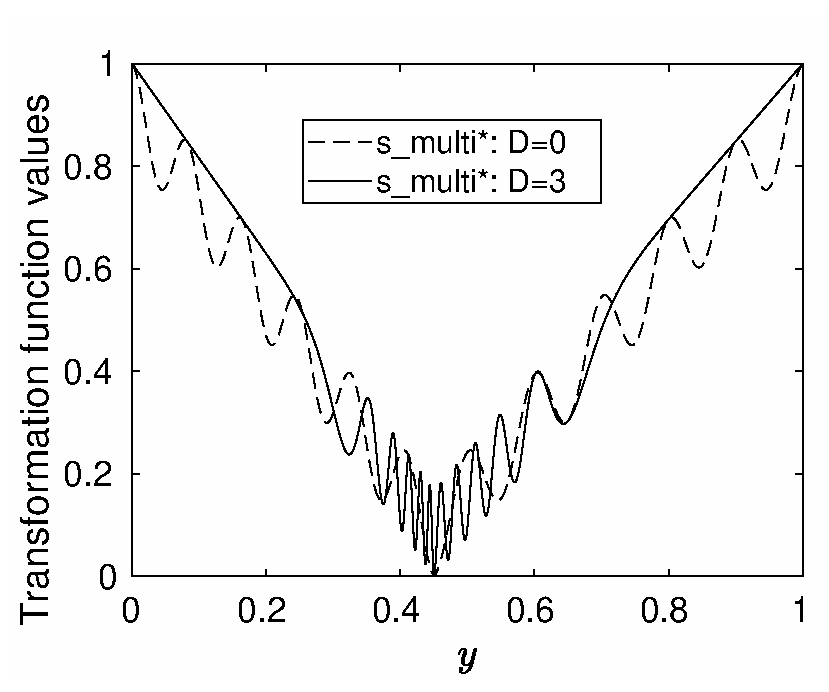
\includegraphics[width=0.31\textwidth]{figures/TestProblemsModality_b.eps}
 \label{fig:transformation_function-b}
}
\subfigure[Proximity to zero]{
 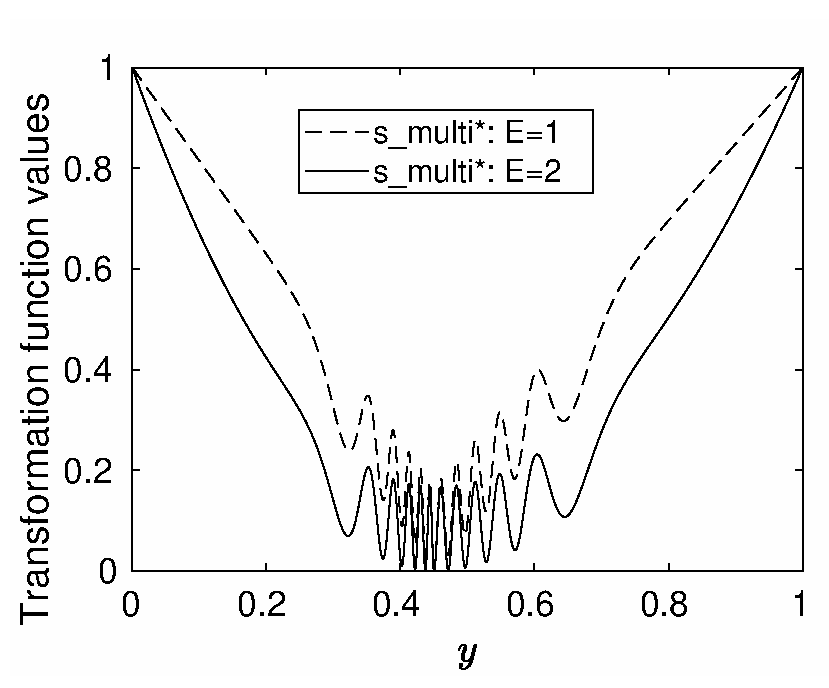
\includegraphics[width=0.31\textwidth]{figures/TestProblemsModality_c.eps}
 \label{fig:transformation_function-c}
}
\subfigure[P1 versus P2]{
 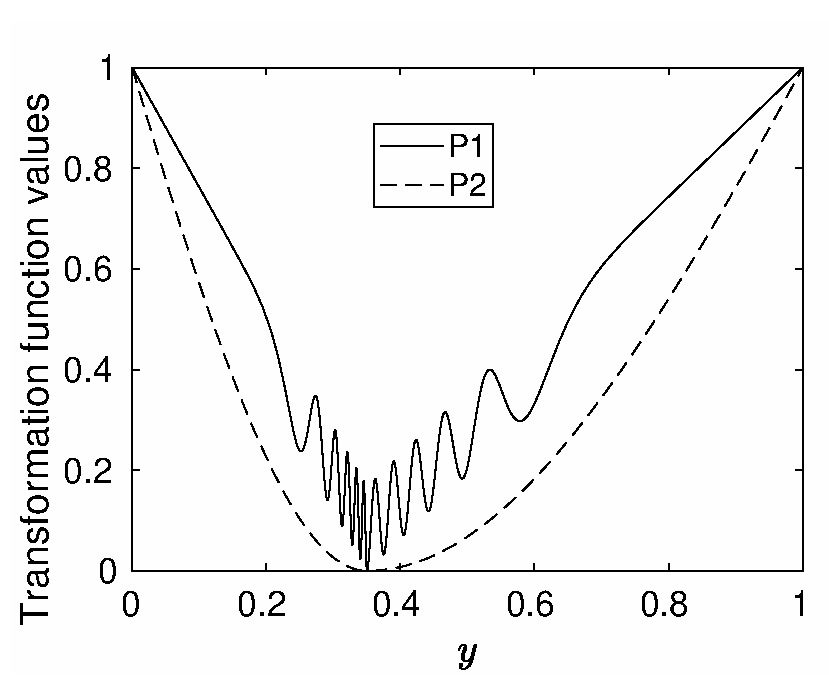
\includegraphics[width=0.31\textwidth]{figures/TestProblems_P1P2Modality.eps}
 \label{fig:transformation_functionP1P2}
}
 \caption{Transformation function in WFG4 as a function of the input parameter ($y$). For (a) and (b) the parameters are $a=5$, $b=10$, and $c=0.35$. The difference between P1 and P2 is shown in (c). Moreover, $e=1$ for (a) and $d=3$ for (b).}
 \label{fig:transformation_function}
\end{figure}

The toolkit from~\cite{Salomon2016Toolkit} is used here to transform the objective vectors of WFG4 into random vectors. The parameters have been chosen to ensure that uncertainty increases towards more optimal regions. The uncertainty also decreases up to a point when moving away from the Pareto region, and then starts increasing again for regions that are further away from the PF. The perturbation is applied to the objective vector by using only its radial component, implying that the perturbation radius is set to zero. This means that an objective vector $\vz$ is perturbed only along one direction, defined by the $n_z-1$ simplex and given by $\hat{\vz} = \vz/\sum z_i$, for $i=1,\ldots,n_z$. In practice, instead of using the deterministic value of the distance term in WFG4, we consider it as a random variate with a uniform distribution. The lower bound of the distribution is situated at the deterministic value from the test problem, and the upper bound increases as solutions approach the Pareto region. As a result, for a given robustness criterion (say, the worst-case scenario as mentioned in Section~\ref{sec:robustness_metric}), the worst performance of the Pareto-optimal solutions can be worse than that of some of the non-Pareto-optimal solutions. This gives rise to the term \textit{Robust Pareto-optimal Set} (RPS), which is defined as the set of solutions with the best performance with respect to the given robustness indicator.

Following the above, we have chosen $c=0.35$ for all test instances. The remaining parameters are: $a=5$, $b=10$, $d=3$, and $e=1$ for P1; and $a=0$, $b=8$, $d=0$, and $e=2$ for P2. The transformation function values for these settings are shown in Figure~\ref{fig:transformation_functionP1P2}. Moreover, the confidence level of the robustness indicator $I_c[S]$ is set to 90\% (i.e., the 90$^\textrm{th}$ percentile of the normal distribution). The PF for P1 corresponds to a quadrant with extremes of 2 and 4 for objectives $f_1$ and $f_2$, respectively, and it is shown in Figure~\ref{fig:reference_sets_p1_PF}. The PF has been obtained by uniformly generating points along the quadrant. Figure~\ref{fig:reference_sets_p2_PF} shows the performance of the RPS with respect to the given robustness indicator. The RPS has been obtained by using an enumeration where the uniform distribution over the distance term of WFG4 has been replaced by the 90$^\textrm{th}$ percentile of the same distribution.

%The obtained PF for P1 and P2 are shown in Figures~\ref{fig:reference_sets_p1_PF} and~\ref{fig:reference_sets_p2_PF}, respectively. The performance set for P1 and P2 have been obtained by fixing the values of the last three decision variables to 2.1, 2.8 and 3.5, respectively, as suggested in the WFG toolkit paper~\cite{bib:wfg_2006}. The values of the first two decision variables have been determined by NSGA-II~\cite{deb2002fast}\footnote{NSGA-II has been run for 10000 generations with the following settings: the distribution index of SBX-crossover and polynomial mutation set to 15 and 20, respectively; and probability of crossover and mutation set to 90\% and 10\%, respectively.} with a population size of 300 solutions, since crowding distance is able to provide a reasonable diverse set across the PF. The robust set for P2 has been obtained by replacing the uniform distribution of the radial component by the 90th percentile of the same distribution (assuming a confidence level of 90\%). NSGA-II is used again with the same settings to determine the values of the decision variables that better satisfy the chosen robustness indicator.

%Notably for P2 as shown in Figure~\ref{fig:reference_sets_p2_PS}, the decision vectors that are Pareto-optimal with respect to the performance criterion are different from the decision vectors that are Pareto-optimal with respect to the robustness criterion. The implication is that an optimal solution set cannot satisfy the performance and robustness criterion simultaneously. Therefore, we use the terms performance PF and robust PF to refer to objective vectors that are Pareto-optimal with respect to either the performance or robustness criterion.

\begin{figure}
\centering
\subfigure[P1]{
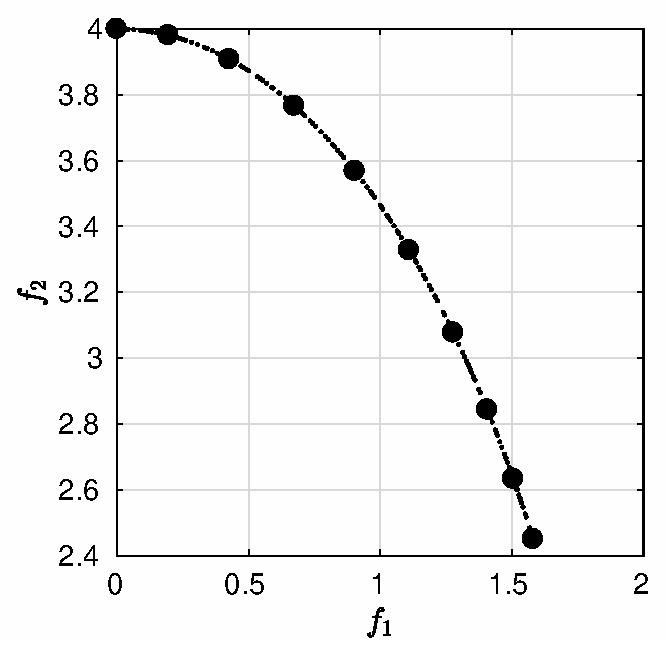
\includegraphics[width=0.3\textwidth]{figures/P1_PF.eps}
\label{fig:reference_sets_p1_PF}
}
\subfigure[P2]{
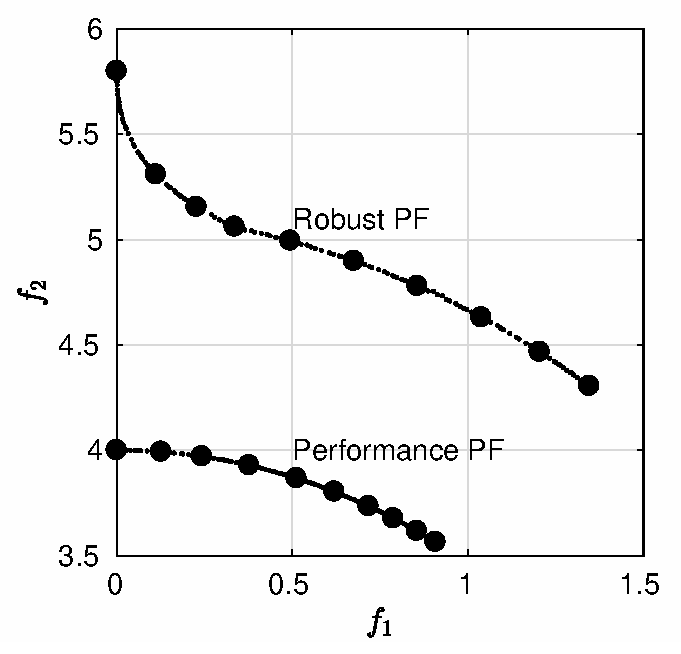
\includegraphics[width=0.3\textwidth]{figures/P2_PF.eps}
\label{fig:reference_sets_p2_PF}
}
\caption{Pareto-optimal front for P1 in (a), and (b) shows the performance of the RPS with respect to the given robustness indicator for P2.}
\label{fig:reference_sets}
\end{figure}


\section{Experimental results}\label{sec:results}

\subsection{Experimental settings}

For both ParEGO and sParEGO algorithms the number of direction vectors is set to 10. Other common parameters are: $n_{init} = 10$, $n_{max} = 50$ and the optimization budget is set to 5000 function evaluations. For sParEGO: $\delta=0.1 \sqrt{n_x}$ and $\delta_{\text{pert}}=\delta / 2$. Inverted Generational Distance (IGD)~\cite{bib:generational_distance} is used to measure the quality of the obtained sets by the optimizers. The 10 solutions that are marked with a filled circle in Figure~\ref{fig:reference_sets} are used as the reference sets for IGD, and these solutions correspond to the best optimal solutions for the chosen direction vectors. 

The optimizers report only one solution per direction vector, implying that only 10 solutions are identified at the end of the optimization process. For each direction vector the solution with the minimum scalarised fitness value is chosen. For this, ParEGO uses the scalarised fitness values determined directly by Equation~\ref{eq:scalarising_function}, while sParEGO uses the fitness attributed by the robustness indicator.

\subsection{Findings}

This section presents the experimental results for problems P1 and P2. The results shown in Figure~\ref{fig:algorithms_comparison} provide both a visual and a analytical assessment of the quality of the solutions obtained by the optimizers in terms of their convergence to and diversity across the PF. The objective vectors for P2 have been determined by evaluating 100 times each decision vector, and the performance of each objective is equal to the 90$^\textrm{th}$ percentile of its marginal distribution.

For P1, ParEGO's approximation to the PF is slightly better than for sParEGO as shown in Figures~\ref{fig:P1_PF_comparison-a} and~\ref{fig:P1_PF_comparison-b}. This indicates that the multi-modality in P1, close to the vinicity of the PF, is interpreted by sParEGO as a region of high uncertainty. The performance of the solutions with respect to the robustness indicator in this region is captured as being poor according to the statistical inferences made by sParEGO. Hence, most sParEGO solutions are just outside the region where the magnitude of the hill sizes of the multi-modality become relatively large. Nevertheless, it is expected for sParEGO to improve its convergence to the PF with more function evaluations, since the statistical assessment made about the true performance of the solutions that are on the PF is also expected to improve.

For P2, sParEGO approximation to the PF obtained with respect to the robustness indicator is better than ParEGO as shown in Figures~\ref{fig:P2_PF_comparison-a} and~\ref{fig:P2_PF_comparison-b}. The convergence of ParEGO deteriorates along the optimization run as shown in Figure~\ref{fig:P2_PF_comparison-b}, while the convergence of sParEGO improves. This indicates that the selection criterion used by ParEGO that promotes solutions with a better nominal performance, leads to a deterioration in the convergence towards the solutions that satisfy the robustness criterion. On the other hand, the uncertainty quantification approach used by sParEGO that is used to estimate the true robustness of the solutions is found to be a better approach in dealing with the task of finding the robust solutions.

\begin{figure}
\centering
\subfigure[P1: Single run (median IGD)]{
 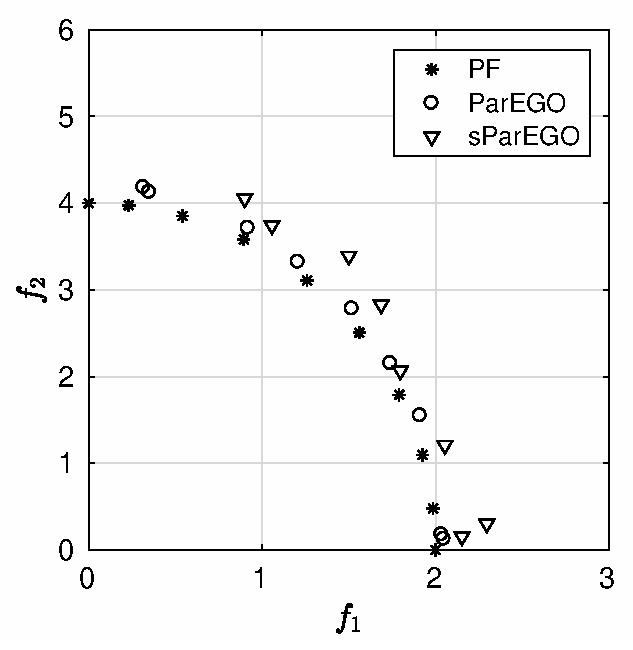
\includegraphics[width=0.3\textwidth]{figures/P1_PF_ParEGO_Vs_sParEGO.eps}
 \label{fig:P1_PF_comparison-a}
}
\hspace{1cm}
\subfigure[P2: Single run (median IGD)]{
 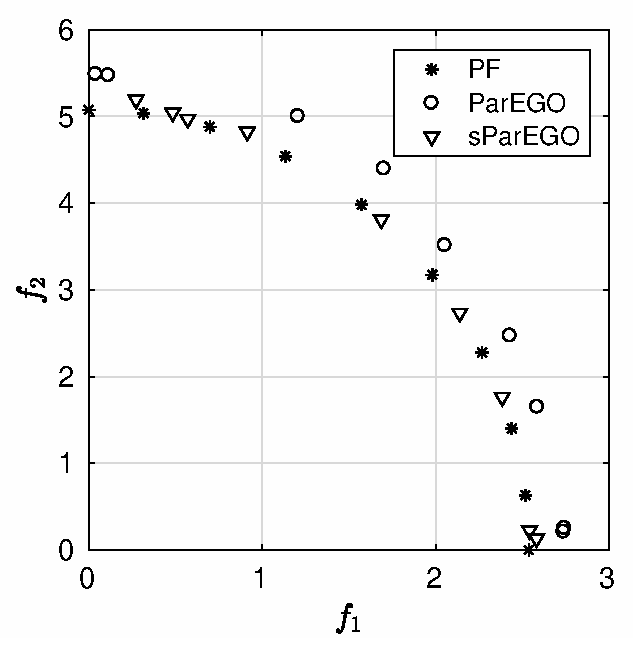
\includegraphics[width=0.3\textwidth]{figures/P2_PF_ParEGO_Vs_sParEGO.eps}
 \label{fig:P2_PF_comparison-a}
}
\\
\subfigure[P1: IGD]{
 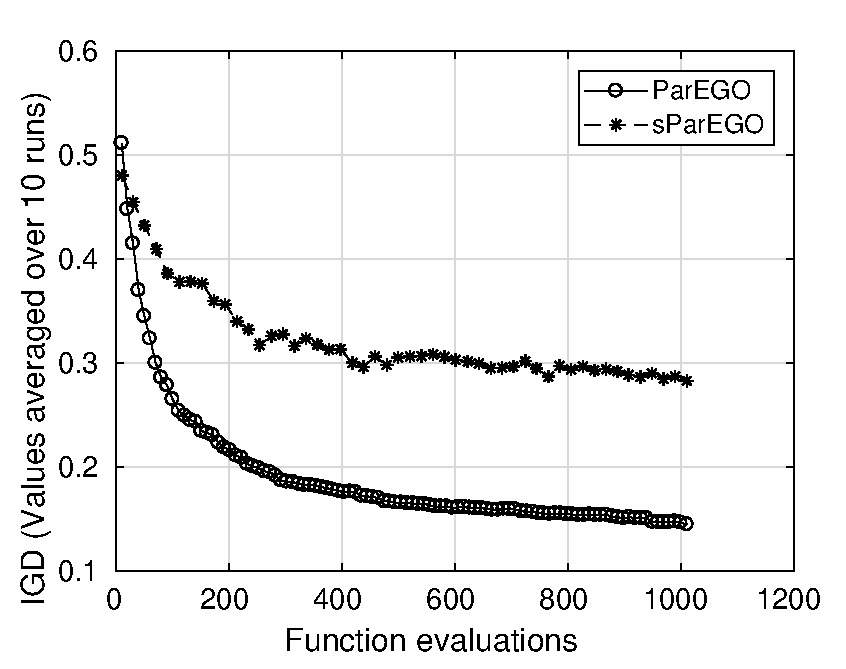
\includegraphics[width=0.33\textwidth]{figures/P1_IGD.eps}
 \label{fig:P1_PF_comparison-b}
}
\hspace{1cm}
\subfigure[P2: IGD]{
 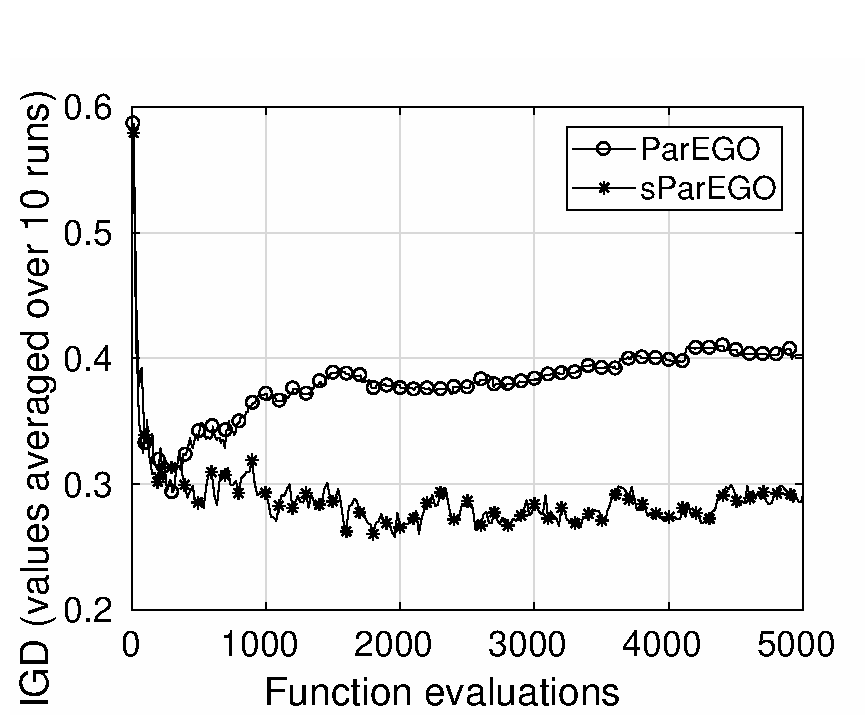
\includegraphics[width=0.33\textwidth]{figures/P2_IGD.eps}
 \label{fig:P2_PF_comparison-b}
}
\caption{Comparison of ParEGO and sParEGO for P1 and P2.}
\label{fig:algorithms_comparison}
\end{figure}

\section{Conclusion}\label{sec:conclusion}

This paper has proposed a new multi-objective optimization algorithm for dealing with expensive uncertain MOPs, namely sParEGO. The comparative analysis with the existing algorithm ParEGO has demonstrated that the statistical inferences made by sParEGO are better equipped to assess the robustness of the candidate solutions for a given robustness criterion. However, we have also shown that the existence of a not-so-well-behaved problem landscape can  mislead the uncertainty quantification approach when (as is necessary) working on a limited budget of evaluations. Given this, the assumptions made within the framework described in this paper, and their associated risks, are as follows:
\begin{enumerate}
 \item \textit{The landscape is well-behaved (i.e.~smooth, continuous)}. The uncertainty distributions are approximated according to available information for other candidate solutions. The underlying assumption for approximating in this way is that similar solutions have similar performance. If the functions are highly ragged and discontinuous, the surrogate models cannot accurately predict their behaviour.
 
 \item \textit{The problem dimensionality is small to medium.} The search is conducted on a surrogate model fitted to the existing evaluated solutions. The surrogate model used in this framework typically produces good estimates for problems with up to 20 design variables.
 
 \item \textit{The maximum distance between solutions to be considered as neighbours, specified by $\delta$, affects the variance of solutions and the convergence rate.} For smooth and continuous functions, a tight neighbourhood is likely to result in smaller variance, but also uses less information from other solutions, which reduces the convergence rate.
\end{enumerate}

Further benchmarking of sParEGO is now needed to confirm its capabilities across a wider set of problem instances. This includes conducting a comparative analysis with other multi-objective robust optimization algorithms, such as those described in the survey in~\cite{bib:robustness_branke_2005}. Other future research directions include: how to approximate the statistical inferences of isolated solutions; how to incorporate constraints; and incorporation of alternative robustness criteria. The source code of the sParEGO algorithm, as well as the test problems, is found within the Liger software, which can be downloaded from the following repository: \url{https://github.com/ligerdev/liger}.

\vspace{2mm}

\textbf{Acknowledgements: }This work was supported by Jaguar Land Rover and the UK-EPSRC grant EP/L025760/1 as part of the jointly funded Programme for Simulation Innovation. The open-source version of Liger was also supported by the Advanced Propulsion Centre UK (grant J14921). The authors acknowledge Joshua Knowles for useful discussions during the design process of sParEGO, and thank all reviewers for their insightful comments and suggestions.

\small{
\bibliographystyle{splncs}
\bibliography{sparegoReferences}
}
\end{document}
